\documentclass{article}

\usepackage[margin=1in]{geometry}
\usepackage{amsmath}
\usepackage{amssymb}
\usepackage{enumitem}
\usepackage{listings}
\usepackage{color}
\usepackage{graphicx}
\usepackage{float}

\graphicspath{{./img/}}

\renewcommand{\lstlistingname}{File}

\definecolor{myblue}{rgb}{0,0,0.5}
\definecolor{myred}{rgb}{0.5,0,0}
\definecolor{mygreen}{rgb}{0,0.5,0}

\lstset{
    language=C,
    basicstyle=\ttfamily\small,
    keywordstyle=\color{myblue},
    stringstyle=\color{myred},
    commentstyle=\color{mygreen},
    frame = single
}

\begin{document}
	{
	\center \Large \textbf{Mobile Robotics Final Exam}\par
	}
	
	\hfill Charlie Coleman
	
	\section*{Question 3}
	
	\subsection*{Straight Wall}
	
	For the straight wall portion of this exam, a simple PD controller was used. Through trial and error, Kp \& Kd values of 0.3 and 9.0 (respectively) were found to give a good result. Loop time was controlled using the onboard timer. A 20ms loop time was not achievable using the 8-bit timer, so a 10ms timer was created and the interrupt system was used to keep track of the number of times the timer reached 10ms. This allowed the loop time to be varied easily. The PD control function for this problem is shown below.
	
	\lstinputlisting[title=Straight Wall PD Controller, firstline=18, lastline=29]{./code/pd.c}
	
	\subsubsection*{20ms Delay}
	
	With a 20ms delay, the robot quickly approaches the wall then quickly levels off around a 0-1" error. 
	
	{\centering
	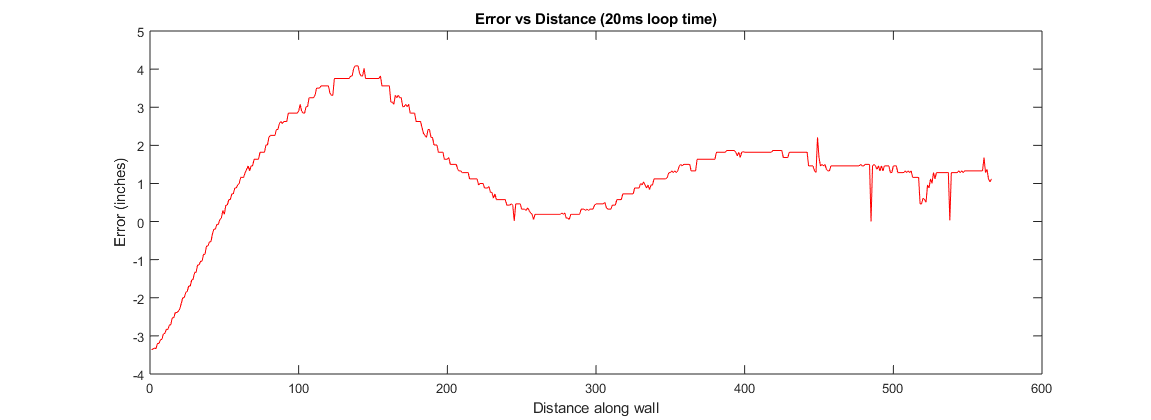
\includegraphics[width=0.9\textwidth]{20msStraightErr}\par
	}
	
	\subsubsection*{10ms Delay}
	
	With a 10ms delay, the robot tends to fluctuate much more, but the error still goes down over time.
	
	{\centering
	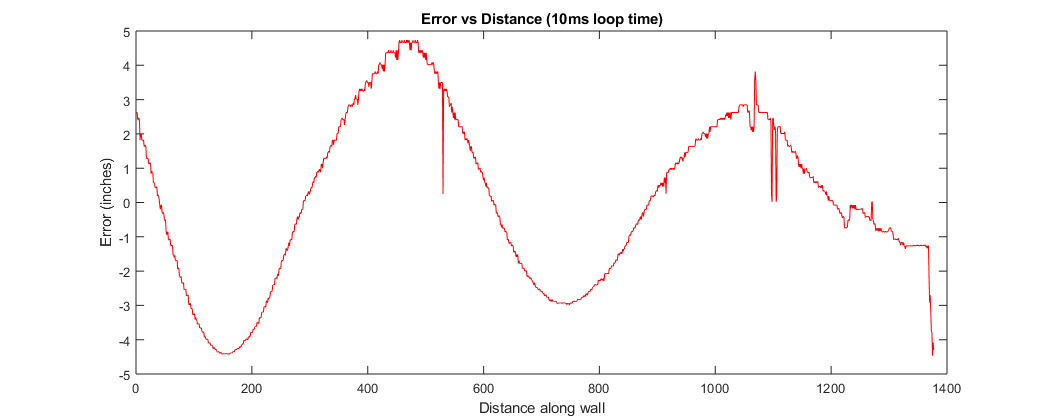
\includegraphics[width=0.9\textwidth]{10msStraightErr}\par
	}
	
	\subsubsection*{40ms Delay}
	
	With a 40ms delay, the path of the robot is much smoother.
	
	{\centering
	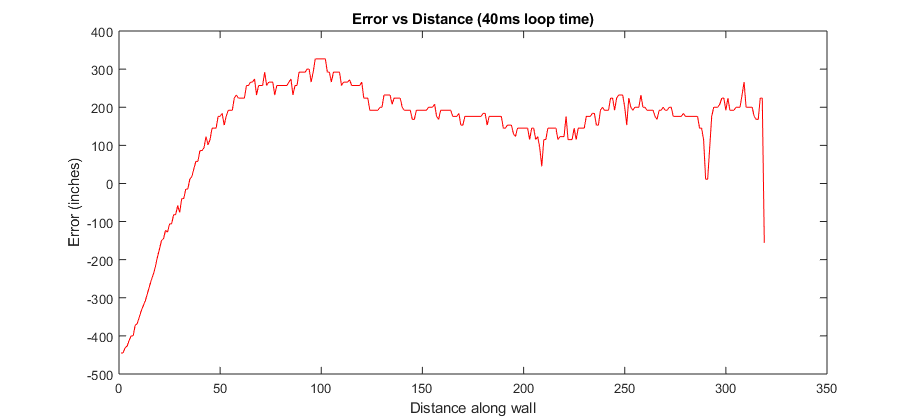
\includegraphics[width=0.9\textwidth]{40msStraightErr}\par
	}
	
	\subsection*{Circular Wall}
	
	I could not find Kp and Kd values that worked for the circular wall, mostly due to time constraints and the fact that it was harder to test this section. An attempted PD controller is shown below.
	
	\lstinputlisting[title=Circular Wall PD Controller, firstline=31, lastline=50]{./code/pd.c}
	
	\subsection*{Outside Corner}
	
	For this problem, I used the same Kp and Kd values from the straight wall portion, but when a sudden change in distance was detected, the Kp and Kd values were changed to much more aggressive values (Kp = 2.0, Kd = 0.15). This allowed the robot to turn sharply until it found the wall. I also found that when the sensor could not accurately find the distance to the wall, the value fluctuated wildly and cause significant errors. In the graph you can see where the corner was reached, as the error jumps to $\approx$160 inches. To prevent this problem, I kept the PD controller input within a specific range. The code for this problem is shown below.
	
	\lstinputlisting[title=Corner Wall PD Controller, firstline=52, lastline=82]{./code/pd.c}
	
	{\centering
	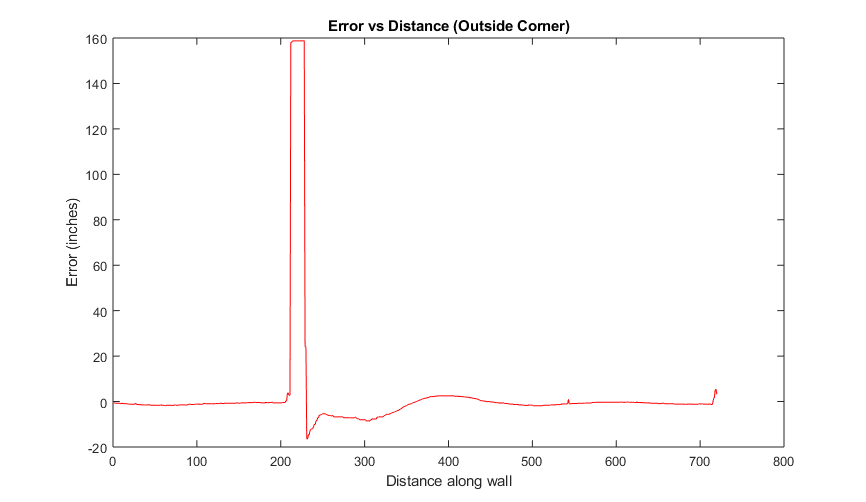
\includegraphics[width=0.9\textwidth]{CornerErr}\par
	}
	
	\section*{Question 4}
	
	For this problem, the code was very similar to the corner wall section of question 3. Instead of changing Kp and Kd a "corner", or sudden change, is detected, we instead increment a counter. When the counter reaches the number of doors we wish to travel past, we turn into the next door using the same aggressive Kp and Kd from the corner section of Q3. For our data, the data did not start collecting soon enough to see the first door, but you can see a sudden \& maintained dip around the 300th sample	. This is the second door as seen by the sensor. Then, the large error seen around 750 is the open door the robot turns into. The code for this problem is shown below.
	
	\lstinputlisting[title=Door PD Controller, firstline=91, lastline=134]{./code/pd.c}
	
	{\centering
	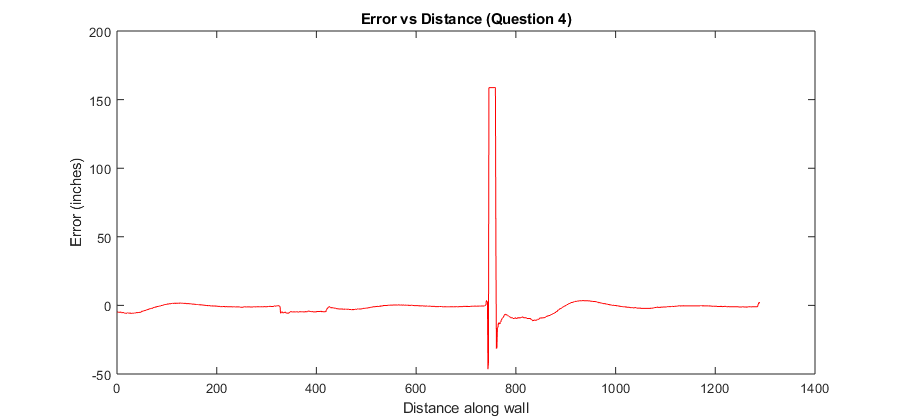
\includegraphics[width=0.9\textwidth]{DoorErr}\par
	}
	
	\pagebreak
	
	\section*{Code}
	
	\lstinputlisting[caption=main.c]{./code/main.c}
	
	\lstinputlisting[caption=serial.h]{./code/serial.h}
	
	\lstinputlisting[caption=serial.c]{./code/serial.c}
	
	\pagebreak
	
	\lstinputlisting[caption=ir.h]{./code/ir.h}
	
	\lstinputlisting[caption=ir.c]{./code/ir.c}
	
	\pagebreak
	
	\lstinputlisting[caption=pwm.h]{./code/pwm.h}
	
	\lstinputlisting[caption=pwm.c]{./code/pwm.c}
	
	\pagebreak
	
	\lstinputlisting[caption=pd.h]{./code/pd.h}
	
	\lstinputlisting[caption=pd.c]{./code/pd.c}
	
	\lstinputlisting[caption=timer.h]{./code/timer.h}
	
	\lstinputlisting[caption=timer.c]{./code/timer.c}
	
\end{document}